% Options for packages loaded elsewhere
\PassOptionsToPackage{unicode}{hyperref}
\PassOptionsToPackage{hyphens}{url}
\PassOptionsToPackage{dvipsnames,svgnames,x11names}{xcolor}
%
\documentclass[
  letterpaper,
  DIV=11,
  numbers=noendperiod]{scrartcl}

\usepackage{amsmath,amssymb}
\usepackage{iftex}
\ifPDFTeX
  \usepackage[T1]{fontenc}
  \usepackage[utf8]{inputenc}
  \usepackage{textcomp} % provide euro and other symbols
\else % if luatex or xetex
  \usepackage{unicode-math}
  \defaultfontfeatures{Scale=MatchLowercase}
  \defaultfontfeatures[\rmfamily]{Ligatures=TeX,Scale=1}
\fi
\usepackage{lmodern}
\ifPDFTeX\else  
    % xetex/luatex font selection
\fi
% Use upquote if available, for straight quotes in verbatim environments
\IfFileExists{upquote.sty}{\usepackage{upquote}}{}
\IfFileExists{microtype.sty}{% use microtype if available
  \usepackage[]{microtype}
  \UseMicrotypeSet[protrusion]{basicmath} % disable protrusion for tt fonts
}{}
\makeatletter
\@ifundefined{KOMAClassName}{% if non-KOMA class
  \IfFileExists{parskip.sty}{%
    \usepackage{parskip}
  }{% else
    \setlength{\parindent}{0pt}
    \setlength{\parskip}{6pt plus 2pt minus 1pt}}
}{% if KOMA class
  \KOMAoptions{parskip=half}}
\makeatother
\usepackage{xcolor}
\setlength{\emergencystretch}{3em} % prevent overfull lines
\setcounter{secnumdepth}{-\maxdimen} % remove section numbering
% Make \paragraph and \subparagraph free-standing
\ifx\paragraph\undefined\else
  \let\oldparagraph\paragraph
  \renewcommand{\paragraph}[1]{\oldparagraph{#1}\mbox{}}
\fi
\ifx\subparagraph\undefined\else
  \let\oldsubparagraph\subparagraph
  \renewcommand{\subparagraph}[1]{\oldsubparagraph{#1}\mbox{}}
\fi

\usepackage{color}
\usepackage{fancyvrb}
\newcommand{\VerbBar}{|}
\newcommand{\VERB}{\Verb[commandchars=\\\{\}]}
\DefineVerbatimEnvironment{Highlighting}{Verbatim}{commandchars=\\\{\}}
% Add ',fontsize=\small' for more characters per line
\usepackage{framed}
\definecolor{shadecolor}{RGB}{241,243,245}
\newenvironment{Shaded}{\begin{snugshade}}{\end{snugshade}}
\newcommand{\AlertTok}[1]{\textcolor[rgb]{0.68,0.00,0.00}{#1}}
\newcommand{\AnnotationTok}[1]{\textcolor[rgb]{0.37,0.37,0.37}{#1}}
\newcommand{\AttributeTok}[1]{\textcolor[rgb]{0.40,0.45,0.13}{#1}}
\newcommand{\BaseNTok}[1]{\textcolor[rgb]{0.68,0.00,0.00}{#1}}
\newcommand{\BuiltInTok}[1]{\textcolor[rgb]{0.00,0.23,0.31}{#1}}
\newcommand{\CharTok}[1]{\textcolor[rgb]{0.13,0.47,0.30}{#1}}
\newcommand{\CommentTok}[1]{\textcolor[rgb]{0.37,0.37,0.37}{#1}}
\newcommand{\CommentVarTok}[1]{\textcolor[rgb]{0.37,0.37,0.37}{\textit{#1}}}
\newcommand{\ConstantTok}[1]{\textcolor[rgb]{0.56,0.35,0.01}{#1}}
\newcommand{\ControlFlowTok}[1]{\textcolor[rgb]{0.00,0.23,0.31}{#1}}
\newcommand{\DataTypeTok}[1]{\textcolor[rgb]{0.68,0.00,0.00}{#1}}
\newcommand{\DecValTok}[1]{\textcolor[rgb]{0.68,0.00,0.00}{#1}}
\newcommand{\DocumentationTok}[1]{\textcolor[rgb]{0.37,0.37,0.37}{\textit{#1}}}
\newcommand{\ErrorTok}[1]{\textcolor[rgb]{0.68,0.00,0.00}{#1}}
\newcommand{\ExtensionTok}[1]{\textcolor[rgb]{0.00,0.23,0.31}{#1}}
\newcommand{\FloatTok}[1]{\textcolor[rgb]{0.68,0.00,0.00}{#1}}
\newcommand{\FunctionTok}[1]{\textcolor[rgb]{0.28,0.35,0.67}{#1}}
\newcommand{\ImportTok}[1]{\textcolor[rgb]{0.00,0.46,0.62}{#1}}
\newcommand{\InformationTok}[1]{\textcolor[rgb]{0.37,0.37,0.37}{#1}}
\newcommand{\KeywordTok}[1]{\textcolor[rgb]{0.00,0.23,0.31}{#1}}
\newcommand{\NormalTok}[1]{\textcolor[rgb]{0.00,0.23,0.31}{#1}}
\newcommand{\OperatorTok}[1]{\textcolor[rgb]{0.37,0.37,0.37}{#1}}
\newcommand{\OtherTok}[1]{\textcolor[rgb]{0.00,0.23,0.31}{#1}}
\newcommand{\PreprocessorTok}[1]{\textcolor[rgb]{0.68,0.00,0.00}{#1}}
\newcommand{\RegionMarkerTok}[1]{\textcolor[rgb]{0.00,0.23,0.31}{#1}}
\newcommand{\SpecialCharTok}[1]{\textcolor[rgb]{0.37,0.37,0.37}{#1}}
\newcommand{\SpecialStringTok}[1]{\textcolor[rgb]{0.13,0.47,0.30}{#1}}
\newcommand{\StringTok}[1]{\textcolor[rgb]{0.13,0.47,0.30}{#1}}
\newcommand{\VariableTok}[1]{\textcolor[rgb]{0.07,0.07,0.07}{#1}}
\newcommand{\VerbatimStringTok}[1]{\textcolor[rgb]{0.13,0.47,0.30}{#1}}
\newcommand{\WarningTok}[1]{\textcolor[rgb]{0.37,0.37,0.37}{\textit{#1}}}

\providecommand{\tightlist}{%
  \setlength{\itemsep}{0pt}\setlength{\parskip}{0pt}}\usepackage{longtable,booktabs,array}
\usepackage{calc} % for calculating minipage widths
% Correct order of tables after \paragraph or \subparagraph
\usepackage{etoolbox}
\makeatletter
\patchcmd\longtable{\par}{\if@noskipsec\mbox{}\fi\par}{}{}
\makeatother
% Allow footnotes in longtable head/foot
\IfFileExists{footnotehyper.sty}{\usepackage{footnotehyper}}{\usepackage{footnote}}
\makesavenoteenv{longtable}
\usepackage{graphicx}
\makeatletter
\def\maxwidth{\ifdim\Gin@nat@width>\linewidth\linewidth\else\Gin@nat@width\fi}
\def\maxheight{\ifdim\Gin@nat@height>\textheight\textheight\else\Gin@nat@height\fi}
\makeatother
% Scale images if necessary, so that they will not overflow the page
% margins by default, and it is still possible to overwrite the defaults
% using explicit options in \includegraphics[width, height, ...]{}
\setkeys{Gin}{width=\maxwidth,height=\maxheight,keepaspectratio}
% Set default figure placement to htbp
\makeatletter
\def\fps@figure{htbp}
\makeatother

\KOMAoption{captions}{tableheading}
\makeatletter
\@ifpackageloaded{caption}{}{\usepackage{caption}}
\AtBeginDocument{%
\ifdefined\contentsname
  \renewcommand*\contentsname{Table of contents}
\else
  \newcommand\contentsname{Table of contents}
\fi
\ifdefined\listfigurename
  \renewcommand*\listfigurename{List of Figures}
\else
  \newcommand\listfigurename{List of Figures}
\fi
\ifdefined\listtablename
  \renewcommand*\listtablename{List of Tables}
\else
  \newcommand\listtablename{List of Tables}
\fi
\ifdefined\figurename
  \renewcommand*\figurename{Figure}
\else
  \newcommand\figurename{Figure}
\fi
\ifdefined\tablename
  \renewcommand*\tablename{Table}
\else
  \newcommand\tablename{Table}
\fi
}
\@ifpackageloaded{float}{}{\usepackage{float}}
\floatstyle{ruled}
\@ifundefined{c@chapter}{\newfloat{codelisting}{h}{lop}}{\newfloat{codelisting}{h}{lop}[chapter]}
\floatname{codelisting}{Listing}
\newcommand*\listoflistings{\listof{codelisting}{List of Listings}}
\makeatother
\makeatletter
\makeatother
\makeatletter
\@ifpackageloaded{caption}{}{\usepackage{caption}}
\@ifpackageloaded{subcaption}{}{\usepackage{subcaption}}
\makeatother
\ifLuaTeX
  \usepackage{selnolig}  % disable illegal ligatures
\fi
\usepackage{bookmark}

\IfFileExists{xurl.sty}{\usepackage{xurl}}{} % add URL line breaks if available
\urlstyle{same} % disable monospaced font for URLs
\hypersetup{
  pdftitle={Test Document},
  pdfauthor={Tiffany Wu},
  colorlinks=true,
  linkcolor={blue},
  filecolor={Maroon},
  citecolor={Blue},
  urlcolor={Blue},
  pdfcreator={LaTeX via pandoc}}

\title{Test Document}
\author{Tiffany Wu}
\date{}

\begin{document}
\maketitle

\subsection{Github Repo Link to Problem Set
1:}\label{github-repo-link-to-problem-set-1}

\url{https://github.com/tiffany-wu/Stats506/tree/82d6a77efe3b9cb471a1524e56975965d28183a4/PS1}

\subsection{Problem 1 - Wine Data}\label{problem-1---wine-data}

\subsubsection{a. Import the data into a data.frame in R. Use the
information in the ``wine.names'' file to give appropriate column names.
(Note: Downloading and unzipping the file can take place outside of your
submitted document, but importing the file should be in the
submission.)}\label{a.-import-the-data-into-a-data.frame-in-r.-use-the-information-in-the-wine.names-file-to-give-appropriate-column-names.-note-downloading-and-unzipping-the-file-can-take-place-outside-of-your-submitted-document-but-importing-the-file-should-be-in-the-submission.}

\begin{Shaded}
\begin{Highlighting}[]
\FunctionTok{rm}\NormalTok{(}\AttributeTok{list =} \FunctionTok{ls}\NormalTok{())}

\CommentTok{\# Import wine data}
\NormalTok{wine }\OtherTok{\textless{}{-}} \FunctionTok{read.csv}\NormalTok{(}\StringTok{"C:/Users/tiffa/University of Michigan Dropbox/Tiffany Wu/Tiffany Wu’s files/Documents/Stats506/PS1/wine.data"}\NormalTok{,}
                 \AttributeTok{header =} \ConstantTok{FALSE}\NormalTok{)}

\CommentTok{\# Rename columns using wine.names file}
\FunctionTok{colnames}\NormalTok{(wine) }\OtherTok{\textless{}{-}} \FunctionTok{c}\NormalTok{(}\StringTok{"Class"}\NormalTok{, }\StringTok{"Alcohol"}\NormalTok{, }\StringTok{"Malic\_Acid"}\NormalTok{, }\StringTok{"Ash"}\NormalTok{, }
                    \StringTok{"Alcalinity\_of\_Ash"}\NormalTok{, }\StringTok{"Magnesium"}\NormalTok{, }\StringTok{"Total\_Phenols"}\NormalTok{, }
                    \StringTok{"Flavanoids"}\NormalTok{, }\StringTok{"Nonflavanoid\_Phenols"}\NormalTok{, }
                    \StringTok{"Proanthocyanins"}\NormalTok{, }\StringTok{"Color\_Intensity"}\NormalTok{, }\StringTok{"Hue"}\NormalTok{, }
                    \StringTok{"Diluted\_Wines"}\NormalTok{, }\StringTok{"Proline"}\NormalTok{)}
\end{Highlighting}
\end{Shaded}

\subsubsection{b. The data contains information on three different
classes of wine. Check and report that the number of wines within each
class is correct as reported in
``wine.names''.}\label{b.-the-data-contains-information-on-three-different-classes-of-wine.-check-and-report-that-the-number-of-wines-within-each-class-is-correct-as-reported-in-wine.names.}

\begin{Shaded}
\begin{Highlighting}[]
\CommentTok{\# Check num of wines in each class}
\CommentTok{\# Should be class 1 59, class 2 71, class 3 48}

\FunctionTok{table}\NormalTok{(wine}\SpecialCharTok{$}\NormalTok{Class)}
\end{Highlighting}
\end{Shaded}

\begin{verbatim}

 1  2  3 
59 71 48 
\end{verbatim}

\subsubsection{c.~Use the data to answer the following
questions:}\label{c.-use-the-data-to-answer-the-following-questions}

\paragraph{1. What is the correlation between alcohol content and color
intensity?}\label{what-is-the-correlation-between-alcohol-content-and-color-intensity}

The correlation is 0.5463642.

\begin{Shaded}
\begin{Highlighting}[]
\CommentTok{\# Corr b/w Alcohol and Color\_Intensity}
\FunctionTok{cor}\NormalTok{(wine}\SpecialCharTok{$}\NormalTok{Alcohol, wine}\SpecialCharTok{$}\NormalTok{Color\_Intensity)}
\end{Highlighting}
\end{Shaded}

\begin{verbatim}
[1] 0.5463642
\end{verbatim}

\paragraph{2. Which class has the highest correlation? Which has the
lowest?}\label{which-class-has-the-highest-correlation-which-has-the-lowest}

Class 1 has the highest correlation, at approximately 0.408. Class 2 has
the lowest correlation, at approximately 0.270.

\begin{Shaded}
\begin{Highlighting}[]
\CommentTok{\# Split the data by class}
\NormalTok{class\_1 }\OtherTok{\textless{}{-}} \FunctionTok{subset}\NormalTok{(wine, Class }\SpecialCharTok{==} \DecValTok{1}\NormalTok{)}
\NormalTok{class\_2 }\OtherTok{\textless{}{-}} \FunctionTok{subset}\NormalTok{(wine, Class }\SpecialCharTok{==} \DecValTok{2}\NormalTok{)}
\NormalTok{class\_3 }\OtherTok{\textless{}{-}} \FunctionTok{subset}\NormalTok{(wine, Class }\SpecialCharTok{==} \DecValTok{3}\NormalTok{)}

\CommentTok{\# Get the correlations for each class}
\NormalTok{cor\_class\_1 }\OtherTok{\textless{}{-}} \FunctionTok{cor}\NormalTok{(class\_1}\SpecialCharTok{$}\NormalTok{Alcohol, class\_1}\SpecialCharTok{$}\NormalTok{Color\_Intensity)}
\NormalTok{cor\_class\_2 }\OtherTok{\textless{}{-}} \FunctionTok{cor}\NormalTok{(class\_2}\SpecialCharTok{$}\NormalTok{Alcohol, class\_2}\SpecialCharTok{$}\NormalTok{Color\_Intensity)}
\NormalTok{cor\_class\_3 }\OtherTok{\textless{}{-}} \FunctionTok{cor}\NormalTok{(class\_3}\SpecialCharTok{$}\NormalTok{Alcohol, class\_3}\SpecialCharTok{$}\NormalTok{Color\_Intensity)}

\CommentTok{\# Show output of all correlations for the html file, don\textquotesingle{}t assign }
\FunctionTok{cor}\NormalTok{(class\_1}\SpecialCharTok{$}\NormalTok{Alcohol, class\_1}\SpecialCharTok{$}\NormalTok{Color\_Intensity)}
\end{Highlighting}
\end{Shaded}

\begin{verbatim}
[1] 0.4082913
\end{verbatim}

\begin{Shaded}
\begin{Highlighting}[]
\FunctionTok{cor}\NormalTok{(class\_2}\SpecialCharTok{$}\NormalTok{Alcohol, class\_2}\SpecialCharTok{$}\NormalTok{Color\_Intensity)}
\end{Highlighting}
\end{Shaded}

\begin{verbatim}
[1] 0.2697891
\end{verbatim}

\begin{Shaded}
\begin{Highlighting}[]
\FunctionTok{cor}\NormalTok{(class\_3}\SpecialCharTok{$}\NormalTok{Alcohol, class\_3}\SpecialCharTok{$}\NormalTok{Color\_Intensity)}
\end{Highlighting}
\end{Shaded}

\begin{verbatim}
[1] 0.3503777
\end{verbatim}

\paragraph{3. What is the alcohol content of the wine with the highest
color
intensity?}\label{what-is-the-alcohol-content-of-the-wine-with-the-highest-color-intensity}

The alcohol content is 14.34.

\begin{Shaded}
\begin{Highlighting}[]
\CommentTok{\# What is the wine with the highest color intensity? Wine 159.}
\NormalTok{max\_color }\OtherTok{\textless{}{-}} \FunctionTok{which.max}\NormalTok{(wine}\SpecialCharTok{$}\NormalTok{Color\_Intensity)}

\CommentTok{\# What is alcohol content for Wine 159?}
\NormalTok{wine}\SpecialCharTok{$}\NormalTok{Alcohol[max\_color]}
\end{Highlighting}
\end{Shaded}

\begin{verbatim}
[1] 14.34
\end{verbatim}

\paragraph{4. What percentage of wines had a higher content of
proanthocyanins compare to
ash?}\label{what-percentage-of-wines-had-a-higher-content-of-proanthocyanins-compare-to-ash}

Approximately 8.43\% of wines had a higher content of proanthocyanins.

\begin{Shaded}
\begin{Highlighting}[]
\CommentTok{\# Number of wines with higher proanthocyanins is 15}
\NormalTok{higher\_p\_count }\OtherTok{\textless{}{-}} \FunctionTok{sum}\NormalTok{(wine}\SpecialCharTok{$}\NormalTok{Proanthocyanins }\SpecialCharTok{\textgreater{}}\NormalTok{ wine}\SpecialCharTok{$}\NormalTok{Ash)}

\CommentTok{\# Divide 15 by total number of wines, multiply by 100 for percentage}
\NormalTok{(higher\_p\_count }\SpecialCharTok{/} \FunctionTok{nrow}\NormalTok{(wine)) }\SpecialCharTok{*} \DecValTok{100}
\end{Highlighting}
\end{Shaded}

\begin{verbatim}
[1] 8.426966
\end{verbatim}

\subsubsection{d.~Create a table identifying the average value of each
variable, providing one row for the overall average, and one row per
class with class averages. (This table does not need to be ``fancy'' but
should clearly identify what each value
represents.)}\label{d.-create-a-table-identifying-the-average-value-of-each-variable-providing-one-row-for-the-overall-average-and-one-row-per-class-with-class-averages.-this-table-does-not-need-to-be-fancy-but-should-clearly-identify-what-each-value-represents.}

\begin{Shaded}
\begin{Highlighting}[]
\CommentTok{\# Get overall average for each column ({-}1 to exclude Class column)}
\NormalTok{overall\_averages }\OtherTok{\textless{}{-}} \FunctionTok{colMeans}\NormalTok{(wine[, }\SpecialCharTok{{-}}\DecValTok{1}\NormalTok{])}

\CommentTok{\# Get the averages for each class}
\NormalTok{class\_1\_avg }\OtherTok{\textless{}{-}} \FunctionTok{colMeans}\NormalTok{(class\_1[, }\SpecialCharTok{{-}}\DecValTok{1}\NormalTok{])}
\NormalTok{class\_2\_avg }\OtherTok{\textless{}{-}} \FunctionTok{colMeans}\NormalTok{(class\_2[, }\SpecialCharTok{{-}}\DecValTok{1}\NormalTok{])}
\NormalTok{class\_3\_avg }\OtherTok{\textless{}{-}} \FunctionTok{colMeans}\NormalTok{(class\_3[, }\SpecialCharTok{{-}}\DecValTok{1}\NormalTok{])}

\CommentTok{\# Combine the averages into a single table}
\NormalTok{average\_table }\OtherTok{\textless{}{-}} \FunctionTok{rbind}\NormalTok{(}
  \AttributeTok{Overall =}\NormalTok{ overall\_averages,}
  \StringTok{"Class 1"} \OtherTok{=}\NormalTok{ class\_1\_avg,}
  \StringTok{"Class\_2"} \OtherTok{=}\NormalTok{ class\_2\_avg,}
  \StringTok{"Class\_3"} \OtherTok{=}\NormalTok{ class\_3\_avg}
\NormalTok{)}

\CommentTok{\# Round}
\NormalTok{average\_table }\OtherTok{\textless{}{-}} \FunctionTok{round}\NormalTok{(average\_table, }\DecValTok{3}\NormalTok{)}

\CommentTok{\# Print table}
\FunctionTok{print}\NormalTok{(average\_table)}
\end{Highlighting}
\end{Shaded}

\begin{verbatim}
        Alcohol Malic_Acid   Ash Alcalinity_of_Ash Magnesium Total_Phenols
Overall  13.001      2.336 2.367            19.495    99.742         2.295
Class 1  13.745      2.011 2.456            17.037   106.339         2.840
Class_2  12.279      1.933 2.245            20.238    94.549         2.259
Class_3  13.154      3.334 2.437            21.417    99.312         1.679
        Flavanoids Nonflavanoid_Phenols Proanthocyanins Color_Intensity   Hue
Overall      2.029                0.362           1.591           5.058 0.957
Class 1      2.982                0.290           1.899           5.528 1.062
Class_2      2.081                0.364           1.630           3.087 1.056
Class_3      0.781                0.448           1.154           7.396 0.683
        Diluted_Wines  Proline
Overall         2.612  746.893
Class 1         3.158 1115.712
Class_2         2.785  519.507
Class_3         1.684  629.896
\end{verbatim}

\begin{Shaded}
\begin{Highlighting}[]
\CommentTok{\# Checking using tidyverse (surpress message, found on StackOverflow)}
\FunctionTok{suppressPackageStartupMessages}\NormalTok{(}\FunctionTok{library}\NormalTok{(tidyverse))}

\CommentTok{\# Overall avg}
\NormalTok{tidy\_avg }\OtherTok{\textless{}{-}}\NormalTok{ wine }\SpecialCharTok{\%\textgreater{}\%}
  \FunctionTok{summarise}\NormalTok{(}\FunctionTok{across}\NormalTok{(}\FunctionTok{where}\NormalTok{(is.numeric), mean))}

\CommentTok{\# For each class}
\NormalTok{class\_averages }\OtherTok{\textless{}{-}}\NormalTok{ wine }\SpecialCharTok{\%\textgreater{}\%}
  \FunctionTok{group\_by}\NormalTok{(Class) }\SpecialCharTok{\%\textgreater{}\%}
  \FunctionTok{summarise}\NormalTok{(}\FunctionTok{across}\NormalTok{(}\FunctionTok{where}\NormalTok{(is.numeric), mean))}
\end{Highlighting}
\end{Shaded}

\subsubsection{e. Carry out a series of t-tests to examine whether the
level of phenols differs across the three classes. Present the R output
and interpret the
results.}\label{e.-carry-out-a-series-of-t-tests-to-examine-whether-the-level-of-phenols-differs-across-the-three-classes.-present-the-r-output-and-interpret-the-results.}

Below I show the t-tests using the \texttt{t.test} function as well as
the manual calculation through creating the function
\texttt{manual\_t\_test}. Overall, all 3 tests show statistically
significant differences in the level of phenols between each pair of
classes. These results suggest that phenol levels differ substantially
across different wine classes.

For the level of phenols between Class 1 and Class 2, the p-value of
1.889e-11 is extremely small, meaning there is a statistically
significant difference between the phenol levels. Additionally, the
confidence interval of {[}0.43, 0.73{]} does not contain 0, further
confirming the statistically significant difference.

For the level of phenols between Class 1 and Class 3, the p-value of
\textless{} 2.2e-16 is also extremely small, meaning there is a
statistically significant difference between the phenol levels.
Additionally, the confidence interval of {[}1.03, 1.30{]} does not
contain 0, further confirming the statistically significant difference.

Lastly, for the level of phenols between Class 2 and Class 3, the
p-value of 1.622e-10 is once again extremely small, meaning there is a
statistically significant difference between the phenol levels.
Additionally, the confidence interval of {[}0.42, 0.72{]} does not
contain 0, further confirming the statistically significant difference.

\begin{Shaded}
\begin{Highlighting}[]
\CommentTok{\# Use existing function just so we can check answer}

\CommentTok{\# Subset the phenol data for each class}
\NormalTok{phenols\_class\_1 }\OtherTok{\textless{}{-}}\NormalTok{ class\_1}\SpecialCharTok{$}\NormalTok{Total\_Phenols}
\NormalTok{phenols\_class\_2 }\OtherTok{\textless{}{-}}\NormalTok{ class\_2}\SpecialCharTok{$}\NormalTok{Total\_Phenols}
\NormalTok{phenols\_class\_3 }\OtherTok{\textless{}{-}}\NormalTok{ class\_3}\SpecialCharTok{$}\NormalTok{Total\_Phenols}

\CommentTok{\# t{-}tests between each pair of classes}
\FunctionTok{t.test}\NormalTok{(phenols\_class\_1, phenols\_class\_2)}
\end{Highlighting}
\end{Shaded}

\begin{verbatim}

    Welch Two Sample t-test

data:  phenols_class_1 and phenols_class_2
t = 7.4206, df = 119.14, p-value = 1.889e-11
alternative hypothesis: true difference in means is not equal to 0
95 percent confidence interval:
 0.4261870 0.7364055
sample estimates:
mean of x mean of y 
 2.840169  2.258873 
\end{verbatim}

\begin{Shaded}
\begin{Highlighting}[]
\FunctionTok{t.test}\NormalTok{(phenols\_class\_1, phenols\_class\_3)}
\end{Highlighting}
\end{Shaded}

\begin{verbatim}

    Welch Two Sample t-test

data:  phenols_class_1 and phenols_class_3
t = 17.12, df = 98.356, p-value < 2.2e-16
alternative hypothesis: true difference in means is not equal to 0
95 percent confidence interval:
 1.026801 1.296038
sample estimates:
mean of x mean of y 
 2.840169  1.678750 
\end{verbatim}

\begin{Shaded}
\begin{Highlighting}[]
\FunctionTok{t.test}\NormalTok{(phenols\_class\_2, phenols\_class\_3)}
\end{Highlighting}
\end{Shaded}

\begin{verbatim}

    Welch Two Sample t-test

data:  phenols_class_2 and phenols_class_3
t = 7.0125, df = 116.91, p-value = 1.622e-10
alternative hypothesis: true difference in means is not equal to 0
95 percent confidence interval:
 0.4162855 0.7439610
sample estimates:
mean of x mean of y 
 2.258873  1.678750 
\end{verbatim}

\subsubsection{For minor extra credit: (You may use an existing R
function to carry out the t-test, or for minor extra credit, manually
write your own calculation of the t-test
p-values.)}\label{for-minor-extra-credit-you-may-use-an-existing-r-function-to-carry-out-the-t-test-or-for-minor-extra-credit-manually-write-your-own-calculation-of-the-t-test-p-values.}

The t-statistic for an independent two-sample t-test, assuming equal
variances is:

\[
t = \frac{\bar{X}_1 - \bar{X}_2}{\sqrt{\frac{s_1^2}{n_1} + \frac{s_2^2}{n_2}}}
\]

Where:

\begin{itemize}
\tightlist
\item
  (\(\bar{X}_1\)) and (\(\bar{X}_2\)) are the sample means of classes 1
  and 2.
\item
  (\(s_1^2\)) and (\(s_2^2\)) are the sample variances of classes 1 and
  2.
\item
  (\(n_1\)) and (\(n_2\)) are the sample sizes of classes 1 and 2.
\end{itemize}

I use the above equation to make my function.

(Attribution of sources: I asked ChatGPT to pull the formula R used for
\texttt{t.test}'s Welch Two Sample t-test, then used ChatGPT again to
write it in LaTeX for RMarkdown. I use the equation pulled to write the
function.)

\begin{Shaded}
\begin{Highlighting}[]
\CommentTok{\# Function to manually calculate t{-}test p{-}value between two samples}
\CommentTok{\# Input takes x and y, both of which are numeric vectors containing the data for the 2 groups we want to compare for the t{-}test}

\CommentTok{\#\textquotesingle{} Manual Welch Two Sample t{-}test}
\CommentTok{\#\textquotesingle{}}
\CommentTok{\#\textquotesingle{} This function performs a Welch Two Sample t{-}test manually. }
\CommentTok{\#\textquotesingle{} }
\CommentTok{\#\textquotesingle{} Used for comparing the means of two independent groups }
\CommentTok{\#\textquotesingle{} while accounting for unequal variances and sample sizes.}
\CommentTok{\#\textquotesingle{}}
\CommentTok{\#\textquotesingle{} @param x Numeric vector representing the first sample.}
\CommentTok{\#\textquotesingle{} @param y Numeric vector representing the second sample.}
\CommentTok{\#\textquotesingle{}}
\CommentTok{\#\textquotesingle{} @return List containing the t{-}statistic and the p{-}value of the test.}
\CommentTok{\#\textquotesingle{} }
\NormalTok{manual\_t\_test }\OtherTok{\textless{}{-}} \ControlFlowTok{function}\NormalTok{(x, y) \{}
  \CommentTok{\# Calculate means}
\NormalTok{  mean\_x }\OtherTok{\textless{}{-}} \FunctionTok{mean}\NormalTok{(x, }\AttributeTok{na.rm =} \ConstantTok{TRUE}\NormalTok{) }\CommentTok{\# check to make sure no NAs}
\NormalTok{  mean\_y }\OtherTok{\textless{}{-}} \FunctionTok{mean}\NormalTok{(y, }\AttributeTok{na.rm =} \ConstantTok{TRUE}\NormalTok{)}
  
  \CommentTok{\# Calculate variances}
\NormalTok{  var\_x }\OtherTok{\textless{}{-}} \FunctionTok{var}\NormalTok{(x, }\AttributeTok{na.rm =} \ConstantTok{TRUE}\NormalTok{)}
\NormalTok{  var\_y }\OtherTok{\textless{}{-}} \FunctionTok{var}\NormalTok{(y, }\AttributeTok{na.rm =} \ConstantTok{TRUE}\NormalTok{)}
  
  \CommentTok{\# Calculate sample sizes}
\NormalTok{  n\_x }\OtherTok{\textless{}{-}} \FunctionTok{length}\NormalTok{(x[}\SpecialCharTok{!}\FunctionTok{is.na}\NormalTok{(x)])}
\NormalTok{  n\_y }\OtherTok{\textless{}{-}} \FunctionTok{length}\NormalTok{(y[}\SpecialCharTok{!}\FunctionTok{is.na}\NormalTok{(y)])}
  
  \CommentTok{\# Calculate the standard error for each group}
\NormalTok{  se\_x }\OtherTok{\textless{}{-}}\NormalTok{ var\_x }\SpecialCharTok{/}\NormalTok{ n\_x}
\NormalTok{  se\_y }\OtherTok{\textless{}{-}}\NormalTok{ var\_y }\SpecialCharTok{/}\NormalTok{ n\_y}
  
  \CommentTok{\# Calculate the t{-}statistic using the Welch formula}
\NormalTok{  t\_stat }\OtherTok{\textless{}{-}}\NormalTok{ (mean\_x }\SpecialCharTok{{-}}\NormalTok{ mean\_y) }\SpecialCharTok{/} \FunctionTok{sqrt}\NormalTok{(se\_x }\SpecialCharTok{+}\NormalTok{ se\_y)}
  
  \CommentTok{\# Calculate degrees of freedom using the Welch formula}
\NormalTok{  df }\OtherTok{\textless{}{-}}\NormalTok{ (se\_x }\SpecialCharTok{+}\NormalTok{ se\_y)}\SpecialCharTok{\^{}}\DecValTok{2} \SpecialCharTok{/}\NormalTok{ ((se\_x}\SpecialCharTok{\^{}}\DecValTok{2}\NormalTok{) }\SpecialCharTok{/}\NormalTok{ (n\_x }\SpecialCharTok{{-}} \DecValTok{1}\NormalTok{) }\SpecialCharTok{+}\NormalTok{ (se\_y}\SpecialCharTok{\^{}}\DecValTok{2}\NormalTok{) }\SpecialCharTok{/}\NormalTok{ (n\_y }\SpecialCharTok{{-}} \DecValTok{1}\NormalTok{))}
  
  \CommentTok{\# Calculate the p{-}value}
  \CommentTok{\# t{-}stat is made negative because pt() func calculates prob of obtaining a value LESS THAN OR EQUAL TO the t{-}stat you give it{-}{-} ensures we look at probability on left tail of distribution}
  \CommentTok{\# Multiply by 2 because t{-}test is two{-}tailed}
\NormalTok{  p\_value }\OtherTok{\textless{}{-}} \DecValTok{2} \SpecialCharTok{*} \FunctionTok{pt}\NormalTok{(}\SpecialCharTok{{-}}\FunctionTok{abs}\NormalTok{(t\_stat), df)}
  
  \CommentTok{\# Return the t{-}statistic and p{-}value}
  \FunctionTok{list}\NormalTok{(}\AttributeTok{t\_statistic =}\NormalTok{ t\_stat, }\AttributeTok{p\_value =}\NormalTok{ p\_value)}
\NormalTok{\}}

\CommentTok{\# Manually perform t{-}tests}
\FunctionTok{manual\_t\_test}\NormalTok{(phenols\_class\_1, phenols\_class\_2)}
\end{Highlighting}
\end{Shaded}

\begin{verbatim}
$t_statistic
[1] 7.420649

$p_value
[1] 1.889329e-11
\end{verbatim}

\begin{Shaded}
\begin{Highlighting}[]
\FunctionTok{manual\_t\_test}\NormalTok{(phenols\_class\_1, phenols\_class\_3)}
\end{Highlighting}
\end{Shaded}

\begin{verbatim}
$t_statistic
[1] 17.12025

$p_value
[1] 2.915038e-31
\end{verbatim}

\begin{Shaded}
\begin{Highlighting}[]
\FunctionTok{manual\_t\_test}\NormalTok{(phenols\_class\_2, phenols\_class\_3)}
\end{Highlighting}
\end{Shaded}

\begin{verbatim}
$t_statistic
[1] 7.012505

$p_value
[1] 1.621575e-10
\end{verbatim}

\subsection{Problem 2 - AskAManager.org
Data}\label{problem-2---askamanager.org-data}

\subsubsection{a. Import the data into a data.frame in R. As with the
wine data, you may download the data outside of your submission, but
importation should take place inside the problem set
submission.}\label{a.-import-the-data-into-a-data.frame-in-r.-as-with-the-wine-data-you-may-download-the-data-outside-of-your-submission-but-importation-should-take-place-inside-the-problem-set-submission.}

\begin{Shaded}
\begin{Highlighting}[]
\NormalTok{askmanager }\OtherTok{\textless{}{-}} \FunctionTok{read.csv}\NormalTok{(}\StringTok{"C:/Users/tiffa/University of Michigan Dropbox/Tiffany Wu/Tiffany Wu’s files/Documents/Stats506/PS1/AskAManager.csv"}\NormalTok{)}
\end{Highlighting}
\end{Shaded}

\subsubsection{b. Clean up the variable names. Simplify
them.}\label{b.-clean-up-the-variable-names.-simplify-them.}

\begin{Shaded}
\begin{Highlighting}[]
\CommentTok{\# Display the original column names to see}
\FunctionTok{print}\NormalTok{(}\FunctionTok{colnames}\NormalTok{(askmanager))}
\end{Highlighting}
\end{Shaded}

\begin{verbatim}
 [1] "X"                                                                                                                                                                                                                                   
 [2] "Timestamp"                                                                                                                                                                                                                           
 [3] "How.old.are.you."                                                                                                                                                                                                                    
 [4] "What.industry.do.you.work.in."                                                                                                                                                                                                       
 [5] "Job.title"                                                                                                                                                                                                                           
 [6] "If.your.job.title.needs.additional.context..please.clarify.here."                                                                                                                                                                    
 [7] "What.is.your.annual.salary...You.ll.indicate.the.currency.in.a.later.question..If.you.are.part.time.or.hourly..please.enter.an.annualized.equivalent....what.you.would.earn.if.you.worked.the.job.40.hours.a.week..52.weeks.a.year.."
 [8] "How.much.additional.monetary.compensation.do.you.get..if.any..for.example..bonuses.or.overtime.in.an.average.year...Please.only.include.monetary.compensation.here..not.the.value.of.benefits."                                      
 [9] "Please.indicate.the.currency"                                                                                                                                                                                                        
[10] "If..Other...please.indicate.the.currency.here.."                                                                                                                                                                                     
[11] "If.your.income.needs.additional.context..please.provide.it.here."                                                                                                                                                                    
[12] "What.country.do.you.work.in."                                                                                                                                                                                                        
[13] "If.you.re.in.the.U.S...what.state.do.you.work.in."                                                                                                                                                                                   
[14] "What.city.do.you.work.in."                                                                                                                                                                                                           
[15] "How.many.years.of.professional.work.experience.do.you.have.overall."                                                                                                                                                                 
[16] "How.many.years.of.professional.work.experience.do.you.have.in.your.field."                                                                                                                                                           
[17] "What.is.your.highest.level.of.education.completed."                                                                                                                                                                                  
[18] "What.is.your.gender."                                                                                                                                                                                                                
[19] "What.is.your.race...Choose.all.that.apply.."                                                                                                                                                                                         
\end{verbatim}

\begin{Shaded}
\begin{Highlighting}[]
\CommentTok{\# Set simplified column names}
\FunctionTok{colnames}\NormalTok{(askmanager) }\OtherTok{\textless{}{-}} \FunctionTok{c}\NormalTok{(}
  \StringTok{"Row"}\NormalTok{, }\StringTok{"Timestamp"}\NormalTok{, }\StringTok{"Age"}\NormalTok{, }\StringTok{"Industry"}\NormalTok{, }\StringTok{"Job\_Title"}\NormalTok{, }
  \StringTok{"Job\_Title\_Context"}\NormalTok{, }\StringTok{"Annual\_Salary"}\NormalTok{, }\StringTok{"Additional\_Compensation"}\NormalTok{, }
  \StringTok{"Currency"}\NormalTok{, }\StringTok{"Currency\_Other"}\NormalTok{, }\StringTok{"Income\_Context"}\NormalTok{, }
  \StringTok{"Country"}\NormalTok{, }\StringTok{"State"}\NormalTok{, }\StringTok{"City"}\NormalTok{, }
  \StringTok{"Years\_Experience\_Total"}\NormalTok{, }\StringTok{"Years\_Experience\_Field"}\NormalTok{, }
  \StringTok{"Education\_Level"}\NormalTok{, }\StringTok{"Gender"}\NormalTok{, }\StringTok{"Race"}
\NormalTok{)}

\CommentTok{\# Display the new column names to verify}
\FunctionTok{print}\NormalTok{(}\FunctionTok{colnames}\NormalTok{(askmanager))}
\end{Highlighting}
\end{Shaded}

\begin{verbatim}
 [1] "Row"                     "Timestamp"              
 [3] "Age"                     "Industry"               
 [5] "Job_Title"               "Job_Title_Context"      
 [7] "Annual_Salary"           "Additional_Compensation"
 [9] "Currency"                "Currency_Other"         
[11] "Income_Context"          "Country"                
[13] "State"                   "City"                   
[15] "Years_Experience_Total"  "Years_Experience_Field" 
[17] "Education_Level"         "Gender"                 
[19] "Race"                   
\end{verbatim}

\subsubsection{c.~Restrict the data to those being paid in US dollars
(USD). Show that it worked by confirming the number of observations
before and after restricting the
data.}\label{c.-restrict-the-data-to-those-being-paid-in-us-dollars-usd.-show-that-it-worked-by-confirming-the-number-of-observations-before-and-after-restricting-the-data.}

Below we show that the number of observations decreased from 28062 to
23374.

\begin{Shaded}
\begin{Highlighting}[]
\CommentTok{\# Number of observations before}
\NormalTok{num\_obs\_b4 }\OtherTok{\textless{}{-}} \FunctionTok{nrow}\NormalTok{(askmanager)}
\NormalTok{num\_obs\_b4}
\end{Highlighting}
\end{Shaded}

\begin{verbatim}
[1] 28062
\end{verbatim}

\begin{Shaded}
\begin{Highlighting}[]
\CommentTok{\# Restrict data}
\NormalTok{us\_dollars }\OtherTok{\textless{}{-}} \FunctionTok{subset}\NormalTok{(askmanager, Currency }\SpecialCharTok{==} \StringTok{"USD"}\NormalTok{)}

\CommentTok{\# Number of observations after}
\NormalTok{num\_obs\_after }\OtherTok{\textless{}{-}} \FunctionTok{nrow}\NormalTok{(us\_dollars)}
\NormalTok{num\_obs\_after}
\end{Highlighting}
\end{Shaded}

\begin{verbatim}
[1] 23374
\end{verbatim}

\subsubsection{d.~Assume no one starts working before age 18. Eliminate
any rows for which their age, years of experience in their field, and
years of experience total are impossible. Again, confirm the number of
observations. (Hint: Making these variables factor may make your life
easier.)}\label{d.-assume-no-one-starts-working-before-age-18.-eliminate-any-rows-for-which-their-age-years-of-experience-in-their-field-and-years-of-experience-total-are-impossible.-again-confirm-the-number-of-observations.-hint-making-these-variables-factor-may-make-your-life-easier.}

For this question, I first eliminated anyone ``Under 18''.

Then, importantly, I assumed that as long as one of the numbers within
each factor combination is possible, we should keep that observation.
For example, you can be ``18-24'' and have ``5-7 years'' for years of
experience because if you are 24 and have 5 years of experience, you
started working at 19, which is valid (even though if you are 18 and
have 5 years of experience that is not valid). As long as there is an
age/experience combination that works, I kept the observation.

After than, I made sure that the years of experience in the field had to
be less than or equal to the years of experience total.

After doing all these subsets, I ended up with 23310 observations (from
23374 after the last question).

\begin{Shaded}
\begin{Highlighting}[]
\CommentTok{\# Number of observations before (after restricting to USD)}
\NormalTok{num\_obs\_b4 }\OtherTok{\textless{}{-}} \FunctionTok{nrow}\NormalTok{(us\_dollars)}
\NormalTok{num\_obs\_b4}
\end{Highlighting}
\end{Shaded}

\begin{verbatim}
[1] 23374
\end{verbatim}

\begin{Shaded}
\begin{Highlighting}[]
\CommentTok{\#  Convert the relevant columns to factor}
\NormalTok{us\_dollars}\SpecialCharTok{$}\NormalTok{Age }\OtherTok{\textless{}{-}} \FunctionTok{as.factor}\NormalTok{(us\_dollars}\SpecialCharTok{$}\NormalTok{Age)}
\NormalTok{us\_dollars}\SpecialCharTok{$}\NormalTok{Years\_Experience\_Total }\OtherTok{\textless{}{-}} \FunctionTok{as.factor}\NormalTok{(us\_dollars}\SpecialCharTok{$}\NormalTok{Years\_Experience\_Total)}
\NormalTok{us\_dollars}\SpecialCharTok{$}\NormalTok{Years\_Experience\_Field }\OtherTok{\textless{}{-}} \FunctionTok{as.factor}\NormalTok{(us\_dollars}\SpecialCharTok{$}\NormalTok{Years\_Experience\_Field)}

\CommentTok{\# See all factor levels}
\FunctionTok{levels}\NormalTok{(us\_dollars}\SpecialCharTok{$}\NormalTok{Age)}
\end{Highlighting}
\end{Shaded}

\begin{verbatim}
[1] "18-24"      "25-34"      "35-44"      "45-54"      "55-64"     
[6] "65 or over" "under 18"  
\end{verbatim}

\begin{Shaded}
\begin{Highlighting}[]
\FunctionTok{levels}\NormalTok{(us\_dollars}\SpecialCharTok{$}\NormalTok{Years\_Experience\_Total)}
\end{Highlighting}
\end{Shaded}

\begin{verbatim}
[1] "1 year or less"   "11 - 20 years"    "2 - 4 years"      "21 - 30 years"   
[5] "31 - 40 years"    "41 years or more" "5-7 years"        "8 - 10 years"    
\end{verbatim}

\begin{Shaded}
\begin{Highlighting}[]
\FunctionTok{levels}\NormalTok{(us\_dollars}\SpecialCharTok{$}\NormalTok{Years\_Experience\_Field)}
\end{Highlighting}
\end{Shaded}

\begin{verbatim}
[1] "1 year or less"   "11 - 20 years"    "2 - 4 years"      "21 - 30 years"   
[5] "31 - 40 years"    "41 years or more" "5-7 years"        "8 - 10 years"    
\end{verbatim}

\begin{Shaded}
\begin{Highlighting}[]
\CommentTok{\# Redo the order because the levels show us it\textquotesingle{}s wrong}
\NormalTok{us\_dollars}\SpecialCharTok{$}\NormalTok{Age }\OtherTok{\textless{}{-}} \FunctionTok{factor}\NormalTok{(us\_dollars}\SpecialCharTok{$}\NormalTok{Age, }
                         \AttributeTok{levels =} \FunctionTok{c}\NormalTok{(}\StringTok{"under 18"}\NormalTok{, }\StringTok{"18{-}24"}\NormalTok{, }\StringTok{"25{-}34"}\NormalTok{, }\StringTok{"35{-}44"}\NormalTok{, }
                                    \StringTok{"45{-}54"}\NormalTok{, }\StringTok{"55{-}64"}\NormalTok{, }\StringTok{"65 or over"}\NormalTok{), }
                         \AttributeTok{ordered =} \ConstantTok{TRUE}\NormalTok{)}

\NormalTok{us\_dollars}\SpecialCharTok{$}\NormalTok{Years\_Experience\_Total }\OtherTok{\textless{}{-}} \FunctionTok{factor}\NormalTok{(us\_dollars}\SpecialCharTok{$}\NormalTok{Years\_Experience\_Total, }
                                            \AttributeTok{levels =} \FunctionTok{c}\NormalTok{(}\StringTok{"1 year or less"}\NormalTok{, }\StringTok{"2 {-} 4 years"}\NormalTok{, }\StringTok{"5{-}7 years"}\NormalTok{, }
                                                       \StringTok{"8 {-} 10 years"}\NormalTok{, }\StringTok{"11 {-} 20 years"}\NormalTok{, }
                                                       \StringTok{"21 {-} 30 years"}\NormalTok{, }\StringTok{"31 {-} 40 years"}\NormalTok{, }
                                                       \StringTok{"41 years or more"}\NormalTok{), }
                                            \AttributeTok{ordered =} \ConstantTok{TRUE}\NormalTok{)}

\NormalTok{us\_dollars}\SpecialCharTok{$}\NormalTok{Years\_Experience\_Field }\OtherTok{\textless{}{-}} \FunctionTok{factor}\NormalTok{(us\_dollars}\SpecialCharTok{$}\NormalTok{Years\_Experience\_Field, }
                                            \AttributeTok{levels =} \FunctionTok{c}\NormalTok{(}\StringTok{"1 year or less"}\NormalTok{, }\StringTok{"2 {-} 4 years"}\NormalTok{, }\StringTok{"5{-}7 years"}\NormalTok{, }
                                                       \StringTok{"8 {-} 10 years"}\NormalTok{, }\StringTok{"11 {-} 20 years"}\NormalTok{, }
                                                       \StringTok{"21 {-} 30 years"}\NormalTok{, }\StringTok{"31 {-} 40 years"}\NormalTok{, }
                                                       \StringTok{"41 years or more"}\NormalTok{), }
                                            \AttributeTok{ordered =} \ConstantTok{TRUE}\NormalTok{)}

\CommentTok{\# Filter out Under 18}
\NormalTok{valid\_rows\_age }\OtherTok{\textless{}{-}} \FunctionTok{subset}\NormalTok{(us\_dollars, }
\NormalTok{                     Age }\SpecialCharTok{!=} \StringTok{"under 18"}\NormalTok{)}

\CommentTok{\# Valid years of experience/age combinations{-}{-} doing unfactored because it\textquotesingle{}s less confusing than keeping track of numbers}
\NormalTok{valid\_rows\_exp }\OtherTok{\textless{}{-}} \FunctionTok{subset}\NormalTok{(valid\_rows\_age, \{}
\NormalTok{  (Age }\SpecialCharTok{==} \StringTok{"18{-}24"} \SpecialCharTok{\&}\NormalTok{ Years\_Experience\_Total }\SpecialCharTok{\%in\%} \FunctionTok{c}\NormalTok{(}\StringTok{"1 year or less"}\NormalTok{, }\StringTok{"2 {-} 4 years"}\NormalTok{, }\StringTok{"5{-}7 years"}\NormalTok{) }\SpecialCharTok{\&}\NormalTok{ Years\_Experience\_Field }\SpecialCharTok{\%in\%} \FunctionTok{c}\NormalTok{(}\StringTok{"1 year or less"}\NormalTok{, }\StringTok{"2 {-} 4 years"}\NormalTok{, }\StringTok{"5{-}7 years"}\NormalTok{)) }\SpecialCharTok{|}
    
\NormalTok{    (Age }\SpecialCharTok{==} \StringTok{"25{-}34"} \SpecialCharTok{\&}\NormalTok{ Years\_Experience\_Total }\SpecialCharTok{\%in\%} \FunctionTok{c}\NormalTok{(}\StringTok{"1 year or less"}\NormalTok{, }\StringTok{"2 {-} 4 years"}\NormalTok{, }\StringTok{"5{-}7 years"}\NormalTok{, }\StringTok{"8 {-} 10 years"}\NormalTok{, }\StringTok{"11 {-} 20 years"}\NormalTok{) }\SpecialCharTok{\&}
\NormalTok{     Years\_Experience\_Field }\SpecialCharTok{\%in\%} \FunctionTok{c}\NormalTok{(}\StringTok{"1 year or less"}\NormalTok{, }\StringTok{"2 {-} 4 years"}\NormalTok{, }\StringTok{"5{-}7 years"}\NormalTok{, }\StringTok{"8 {-} 10 years"}\NormalTok{, }\StringTok{"11 {-} 20 years"}\NormalTok{)) }\SpecialCharTok{|}
    
\NormalTok{  (Age }\SpecialCharTok{==} \StringTok{"35{-}44"} \SpecialCharTok{\&}\NormalTok{ Years\_Experience\_Total }\SpecialCharTok{\%in\%} \FunctionTok{c}\NormalTok{(}\StringTok{"1 year or less"}\NormalTok{, }\StringTok{"2 {-} 4 years"}\NormalTok{, }\StringTok{"5{-}7 years"}\NormalTok{, }\StringTok{"8 {-} 10 years"}\NormalTok{, }\StringTok{"11 {-} 20 years"}\NormalTok{, }\StringTok{"21 {-} 30 years"}\NormalTok{) }\SpecialCharTok{\&}
\NormalTok{     Years\_Experience\_Field }\SpecialCharTok{\%in\%} \FunctionTok{c}\NormalTok{(}\StringTok{"1 year or less"}\NormalTok{, }\StringTok{"2 {-} 4 years"}\NormalTok{, }\StringTok{"5{-}7 years"}\NormalTok{, }\StringTok{"8 {-} 10 years"}\NormalTok{, }\StringTok{"11 {-} 20 years"}\NormalTok{, }\StringTok{"21 {-} 30 years"}\NormalTok{)) }\SpecialCharTok{|}
    
\NormalTok{  (Age }\SpecialCharTok{==} \StringTok{"45{-}54"} \SpecialCharTok{\&}\NormalTok{ Years\_Experience\_Total }\SpecialCharTok{\%in\%} \FunctionTok{c}\NormalTok{(}\StringTok{"1 year or less"}\NormalTok{, }\StringTok{"2 {-} 4 years"}\NormalTok{, }\StringTok{"5{-}7 years"}\NormalTok{, }\StringTok{"8 {-} 10 years"}\NormalTok{, }\StringTok{"11 {-} 20 years"}\NormalTok{, }\StringTok{"21 {-} 30 years"}\NormalTok{, }\StringTok{"31 {-} 40 years"}\NormalTok{) }\SpecialCharTok{\&}
\NormalTok{     Years\_Experience\_Field }\SpecialCharTok{\%in\%} \FunctionTok{c}\NormalTok{(}\StringTok{"1 year or less"}\NormalTok{, }\StringTok{"2 {-} 4 years"}\NormalTok{, }\StringTok{"5{-}7 years"}\NormalTok{, }\StringTok{"8 {-} 10 years"}\NormalTok{, }\StringTok{"11 {-} 20 years"}\NormalTok{, }\StringTok{"21 {-} 30 years"}\NormalTok{, }\StringTok{"31 {-} 40 years"}\NormalTok{)) }\SpecialCharTok{|}
    
\NormalTok{  (Age }\SpecialCharTok{==} \StringTok{"55{-}64"} \SpecialCharTok{\&}\NormalTok{ Years\_Experience\_Total }\SpecialCharTok{\%in\%} \FunctionTok{c}\NormalTok{(}\StringTok{"1 year or less"}\NormalTok{, }\StringTok{"2 {-} 4 years"}\NormalTok{, }\StringTok{"5{-}7 years"}\NormalTok{, }\StringTok{"8 {-} 10 years"}\NormalTok{, }\StringTok{"11 {-} 20 years"}\NormalTok{,}\StringTok{"21 {-} 30 years"}\NormalTok{, }\StringTok{"31 {-} 40 years"}\NormalTok{, }\StringTok{"41 years or more"}\NormalTok{) }\SpecialCharTok{\&}
\NormalTok{     Years\_Experience\_Field }\SpecialCharTok{\%in\%} \FunctionTok{c}\NormalTok{(}\StringTok{"1 year or less"}\NormalTok{, }\StringTok{"2 {-} 4 years"}\NormalTok{, }\StringTok{"5{-}7 years"}\NormalTok{, }\StringTok{"8 {-} 10 years"}\NormalTok{, }\StringTok{"11 {-} 20 years"}\NormalTok{,}\StringTok{"21 {-} 30 years"}\NormalTok{, }\StringTok{"31 {-} 40 years"}\NormalTok{, }\StringTok{"41 years or more"}\NormalTok{)) }\SpecialCharTok{|}
    
\NormalTok{  (Age }\SpecialCharTok{==} \StringTok{"65 or over"} \SpecialCharTok{\&}\NormalTok{ Years\_Experience\_Total }\SpecialCharTok{\%in\%} \FunctionTok{c}\NormalTok{(}\StringTok{"1 year or less"}\NormalTok{, }\StringTok{"2 {-} 4 years"}\NormalTok{, }\StringTok{"5{-}7 years"}\NormalTok{, }\StringTok{"8 {-} 10 years"}\NormalTok{, }\StringTok{"11 {-} 20 years"}\NormalTok{,}\StringTok{"21 {-} 30 years"}\NormalTok{, }\StringTok{"31 {-} 40 years"}\NormalTok{, }\StringTok{"41 years or more"}\NormalTok{) }\SpecialCharTok{\&}
\NormalTok{     Years\_Experience\_Field }\SpecialCharTok{\%in\%} \FunctionTok{c}\NormalTok{(}\StringTok{"1 year or less"}\NormalTok{, }\StringTok{"2 {-} 4 years"}\NormalTok{, }\StringTok{"5{-}7 years"}\NormalTok{, }\StringTok{"8 {-} 10 years"}\NormalTok{, }\StringTok{"11 {-} 20 years"}\NormalTok{,}\StringTok{"21 {-} 30 years"}\NormalTok{, }\StringTok{"31 {-} 40 years"}\NormalTok{, }\StringTok{"41 years or more"}\NormalTok{)) }\SpecialCharTok{\&}
    \CommentTok{\# Can\textquotesingle{}t have more years of experience in field than years of experience total, use factors here}
\NormalTok{  (}\FunctionTok{as.numeric}\NormalTok{(Years\_Experience\_Total) }\SpecialCharTok{\textgreater{}=} \FunctionTok{as.numeric}\NormalTok{(Years\_Experience\_Field))}
\NormalTok{\})}

\CommentTok{\# Number of observations after}
\NormalTok{num\_obs\_after }\OtherTok{\textless{}{-}} \FunctionTok{nrow}\NormalTok{(valid\_rows\_exp)}
\NormalTok{num\_obs\_after}
\end{Highlighting}
\end{Shaded}

\begin{verbatim}
[1] 23310
\end{verbatim}

\subsubsection{e. A lot of the incomes are likely false. Eliminate any
rows with extremely low or extremely high salaries. I'll leave the
decision of what thresholds to use up to you; you could choose to
eliminate only impossible values, or you could restrict the sample to
eliminate the extreme values even if they are realistic (e.g.~removing
the billionaires or the folks making \textless{} \$1,000 per year). You
must justify your choice, along with either a cited source or an
exploration the data, or some combination.Report your final sample
size.}\label{e.-a-lot-of-the-incomes-are-likely-false.-eliminate-any-rows-with-extremely-low-or-extremely-high-salaries.-ill-leave-the-decision-of-what-thresholds-to-use-up-to-you-you-could-choose-to-eliminate-only-impossible-values-or-you-could-restrict-the-sample-to-eliminate-the-extreme-values-even-if-they-are-realistic-e.g.-removing-the-billionaires-or-the-folks-making-1000-per-year.-you-must-justify-your-choice-along-with-either-a-cited-source-or-an-exploration-the-data-or-some-combination.report-your-final-sample-size.}

The timestamp on the AskaManager.org dataframe is in the year 2021-2022
in the U.S. Looking at both websites (linked) on
\href{https://www.census.gov/library/publications/2023/demo/p60-279.html}{census.gov}
and
\href{https://www.statista.com/statistics/203183/percentage-distribution-of-household-income-in-the-us/}{statista.com},
we see that the median household income was a little under \$75,000 in
2022. By plotting both a histogram and a boxplot to explore the data, we
see that the distribution of the income in our data is positive skewed,
and there are quite a few outlier observations making a lot more money
than the average person in the U.S. in this time frame.

Our strategy to restrict the sample was to eliminate the extreme low
values first by removing those making \textless{} \$1000 per year unless
they had a non-0, more than 1000, non-NA value in the
Additional\_Compensation column. If they had additional compensation
greater than 1000 USD, we assumed they had enough money for it to be
realistic. Then, we remove the billionaire outlier (income of
102000000). The median income in this dataset after those removals was
78551 USD, which is a little higher than the median household income we
got looking at the sources above, but it is very close. Because of this,
we decide to keep all remaining observations.

The resulting dataframe has 23247 observations.

\begin{Shaded}
\begin{Highlighting}[]
\CommentTok{\# Rename from last question}
\NormalTok{us\_dollars\_salary }\OtherTok{\textless{}{-}}\NormalTok{ valid\_rows\_exp}

\CommentTok{\# Plot Annual Salary distribution}

\CommentTok{\# Histogram, 14 rows greater than 1 mil}
\NormalTok{us\_dollars\_salary }\SpecialCharTok{\%\textgreater{}\%}
  \FunctionTok{ggplot}\NormalTok{(}\FunctionTok{aes}\NormalTok{(}\AttributeTok{x =}\NormalTok{ Annual\_Salary)) }\SpecialCharTok{+}
  \FunctionTok{geom\_histogram}\NormalTok{(}\AttributeTok{bins =} \DecValTok{50}\NormalTok{, }\AttributeTok{fill =} \StringTok{"lightblue"}\NormalTok{, }\AttributeTok{color =} \StringTok{"black"}\NormalTok{) }\SpecialCharTok{+}
  \FunctionTok{labs}\NormalTok{(}
    \AttributeTok{title =} \StringTok{"Distribution of Annual Salary"}\NormalTok{,}
    \AttributeTok{x =} \StringTok{"Annual Salary (USD)"}\NormalTok{,}
    \AttributeTok{y =} \StringTok{"Frequency"}
\NormalTok{  ) }\SpecialCharTok{+}
  \FunctionTok{xlim}\NormalTok{(}\DecValTok{0}\NormalTok{, }\DecValTok{1000000}\NormalTok{) }\SpecialCharTok{+} 
  \FunctionTok{theme\_minimal}\NormalTok{()}
\end{Highlighting}
\end{Shaded}

\begin{verbatim}
Warning: Removed 14 rows containing non-finite outside the scale range
(`stat_bin()`).
\end{verbatim}

\begin{verbatim}
Warning: Removed 2 rows containing missing values or values outside the scale range
(`geom_bar()`).
\end{verbatim}

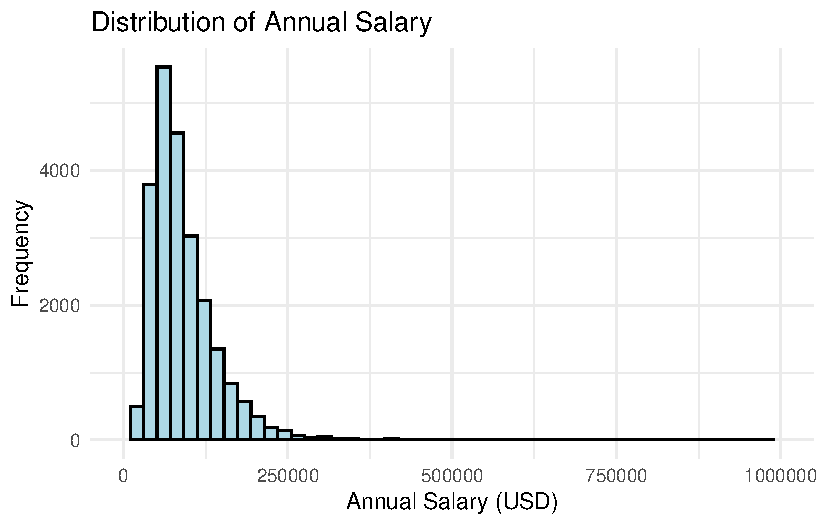
\includegraphics{PS1_files/figure-pdf/unnamed-chunk-15-1.pdf}

\begin{Shaded}
\begin{Highlighting}[]
\CommentTok{\# Boxplot to help identify outliers, 14 rows greater than 1 mil}
\NormalTok{us\_dollars\_salary }\SpecialCharTok{\%\textgreater{}\%}
  \FunctionTok{ggplot}\NormalTok{(}\FunctionTok{aes}\NormalTok{(}\AttributeTok{y =}\NormalTok{ Annual\_Salary)) }\SpecialCharTok{+}
  \FunctionTok{geom\_boxplot}\NormalTok{(}\AttributeTok{fill =} \StringTok{"lightgreen"}\NormalTok{, }\AttributeTok{color =} \StringTok{"black"}\NormalTok{) }\SpecialCharTok{+}
  \FunctionTok{labs}\NormalTok{(}
    \AttributeTok{title =} \StringTok{"Boxplot of Annual Salary"}\NormalTok{,}
    \AttributeTok{y =} \StringTok{"Annual Salary (USD)"}
\NormalTok{  ) }\SpecialCharTok{+}
  \FunctionTok{ylim}\NormalTok{(}\DecValTok{0}\NormalTok{, }\DecValTok{1000000}\NormalTok{) }\SpecialCharTok{+} \CommentTok{\# Adjust as needed for better visualization}
  \FunctionTok{theme\_minimal}\NormalTok{()}
\end{Highlighting}
\end{Shaded}

\begin{verbatim}
Warning: Removed 14 rows containing non-finite outside the scale range
(`stat_boxplot()`).
\end{verbatim}

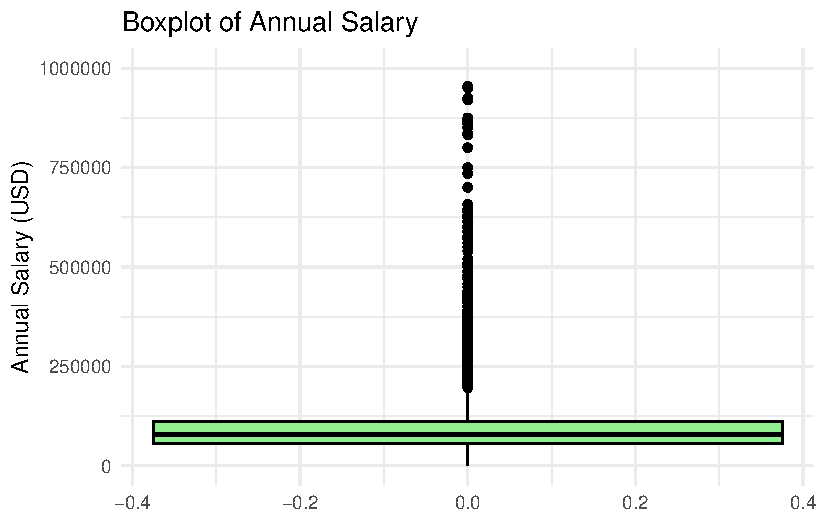
\includegraphics{PS1_files/figure-pdf/unnamed-chunk-15-2.pdf}

\begin{Shaded}
\begin{Highlighting}[]
\CommentTok{\# Omit NAs{-}{-} no NAs in Annual\_Salary column}
\NormalTok{us\_dollars\_salary }\OtherTok{\textless{}{-}} \FunctionTok{subset}\NormalTok{(us\_dollars, }\SpecialCharTok{!}\FunctionTok{is.na}\NormalTok{(Annual\_Salary))}

\CommentTok{\# Remove those making \textless{} $1000 per year unless they had additional compensation following above rules}
\NormalTok{us\_dollars\_salary2 }\OtherTok{\textless{}{-}}\NormalTok{ us\_dollars\_salary[}
  \SpecialCharTok{!}\NormalTok{(us\_dollars\_salary}\SpecialCharTok{$}\NormalTok{Annual\_Salary }\SpecialCharTok{\textless{}} \DecValTok{1000} \SpecialCharTok{\&} 
\NormalTok{    (}\FunctionTok{is.na}\NormalTok{(us\_dollars\_salary}\SpecialCharTok{$}\NormalTok{Additional\_Compensation) }\SpecialCharTok{|}
\NormalTok{       us\_dollars\_salary}\SpecialCharTok{$}\NormalTok{Additional\_Compensation }\SpecialCharTok{\textless{}} \DecValTok{1000}\NormalTok{)), }
\NormalTok{]}

\CommentTok{\# Remove specific  billionaire outlier}
\NormalTok{us\_dollars\_salary3 }\OtherTok{\textless{}{-}}\NormalTok{ us\_dollars\_salary2[}
  \SpecialCharTok{!}\NormalTok{(us\_dollars\_salary2}\SpecialCharTok{$}\NormalTok{Annual\_Salary }\SpecialCharTok{==} \DecValTok{102000000}\NormalTok{), }
\NormalTok{]}

\CommentTok{\# Get max and min}
\FunctionTok{max}\NormalTok{(us\_dollars\_salary3}\SpecialCharTok{$}\NormalTok{Annual\_Salary)}
\end{Highlighting}
\end{Shaded}

\begin{verbatim}
[1] 1e+07
\end{verbatim}

\begin{Shaded}
\begin{Highlighting}[]
\FunctionTok{min}\NormalTok{(us\_dollars\_salary3}\SpecialCharTok{$}\NormalTok{Annual\_Salary)}
\end{Highlighting}
\end{Shaded}

\begin{verbatim}
[1] 0
\end{verbatim}

\begin{Shaded}
\begin{Highlighting}[]
\FunctionTok{median}\NormalTok{(us\_dollars\_salary3}\SpecialCharTok{$}\NormalTok{Annual\_Salary)}
\end{Highlighting}
\end{Shaded}

\begin{verbatim}
[1] 78560
\end{verbatim}

\begin{Shaded}
\begin{Highlighting}[]
\CommentTok{\# Get number of observations}
\FunctionTok{nrow}\NormalTok{(us\_dollars\_salary3)}
\end{Highlighting}
\end{Shaded}

\begin{verbatim}
[1] 23307
\end{verbatim}

\subsubsection{f.~(Optional) If you want to see this analysis through
for no credit, answer the research question of whether there is a
statistical association between education and salary, controlling for
years of
experience.}\label{f.-optional-if-you-want-to-see-this-analysis-through-for-no-credit-answer-the-research-question-of-whether-there-is-a-statistical-association-between-education-and-salary-controlling-for-years-of-experience.}

First, we convert the years of experience variables into numeric and get
the correlation between years of experience total and years of
experience in the field to see if we should include both variables in
our regression model. Since the correlation is 0.7601124, which is
pretty high, we decide to just use the total years of experience
variable.

Controlling for years of total experience, we do see a statistically
significant association between education and salary. Of course, we are
not including all possible confounding factors into our regression
model, so we can't make any causal conclusions.

\begin{Shaded}
\begin{Highlighting}[]
\CommentTok{\# Create a df that converts factors to numbers}
\NormalTok{us\_dollars\_nums }\OtherTok{\textless{}{-}}\NormalTok{ us\_dollars\_salary3}

\CommentTok{\# Convert factors to numeric values}
\NormalTok{us\_dollars\_nums}\SpecialCharTok{$}\NormalTok{Years\_Experience\_Total }\OtherTok{\textless{}{-}} \FunctionTok{as.numeric}\NormalTok{((us\_dollars\_salary3}\SpecialCharTok{$}\NormalTok{Years\_Experience\_Total))}
\NormalTok{us\_dollars\_nums}\SpecialCharTok{$}\NormalTok{Years\_Experience\_Field }\OtherTok{\textless{}{-}} \FunctionTok{as.numeric}\NormalTok{((us\_dollars\_salary3}\SpecialCharTok{$}\NormalTok{Years\_Experience\_Field))}

\CommentTok{\# Correlation}
\FunctionTok{cor}\NormalTok{(us\_dollars\_nums}\SpecialCharTok{$}\NormalTok{Years\_Experience\_Total, us\_dollars\_nums}\SpecialCharTok{$}\NormalTok{Years\_Experience\_Field,}
    \AttributeTok{use =} \StringTok{"complete.obs"}\NormalTok{)}
\end{Highlighting}
\end{Shaded}

\begin{verbatim}
[1] 0.7550524
\end{verbatim}

\begin{Shaded}
\begin{Highlighting}[]
\FunctionTok{library}\NormalTok{(lmtest)}
\end{Highlighting}
\end{Shaded}

\begin{verbatim}
Loading required package: zoo
\end{verbatim}

\begin{verbatim}

Attaching package: 'zoo'
\end{verbatim}

\begin{verbatim}
The following objects are masked from 'package:base':

    as.Date, as.Date.numeric
\end{verbatim}

\begin{Shaded}
\begin{Highlighting}[]
\CommentTok{\# Fit regression}
\NormalTok{salary\_model }\OtherTok{\textless{}{-}} \FunctionTok{lm}\NormalTok{(Annual\_Salary }\SpecialCharTok{\textasciitilde{}}\NormalTok{ Education\_Level }\SpecialCharTok{+}\NormalTok{ Years\_Experience\_Total,}
                   \AttributeTok{data =}\NormalTok{ us\_dollars\_salary3)}

\CommentTok{\# Display the summary of the model}
\NormalTok{summary\_lm }\OtherTok{\textless{}{-}} \FunctionTok{summary}\NormalTok{(salary\_model)}

\FunctionTok{print}\NormalTok{(summary\_lm)}
\end{Highlighting}
\end{Shaded}

\begin{verbatim}

Call:
lm(formula = Annual_Salary ~ Education_Level + Years_Experience_Total, 
    data = us_dollars_salary3)

Residuals:
    Min      1Q  Median      3Q     Max 
-179087  -32435  -11950   17907 9750913 

Coefficients:
                                                  Estimate Std. Error t value
(Intercept)                                       125030.4     8403.1  14.879
Education_LevelCollege degree                     -26737.6     8344.2  -3.204
Education_LevelHigh School                        -33864.7     9702.0  -3.490
Education_LevelMaster's degree                    -23451.5     8373.1  -2.801
Education_LevelPhD                                 -3083.8     8825.1  -0.349
Education_LevelProfessional degree (MD, JD, etc.)  36061.4     8821.1   4.088
Education_LevelSome college                       -42745.3     8674.4  -4.928
Years_Experience_Total.L                           89271.2     6152.3  14.510
Years_Experience_Total.Q                           36745.7     5963.4   6.162
Years_Experience_Total.C                           26451.8     4992.5   5.298
Years_Experience_Total^4                           22636.0     3877.5   5.838
Years_Experience_Total^5                           11475.6     2878.6   3.987
Years_Experience_Total^6                            6932.9     2091.8   3.314
Years_Experience_Total^7                             743.2     1535.2   0.484
                                                  Pr(>|t|)    
(Intercept)                                        < 2e-16 ***
Education_LevelCollege degree                     0.001356 ** 
Education_LevelHigh School                        0.000483 ***
Education_LevelMaster's degree                    0.005101 ** 
Education_LevelPhD                                0.726768    
Education_LevelProfessional degree (MD, JD, etc.) 4.36e-05 ***
Education_LevelSome college                       8.38e-07 ***
Years_Experience_Total.L                           < 2e-16 ***
Years_Experience_Total.Q                          7.30e-10 ***
Years_Experience_Total.C                          1.18e-07 ***
Years_Experience_Total^4                          5.36e-09 ***
Years_Experience_Total^5                          6.72e-05 ***
Years_Experience_Total^6                          0.000920 ***
Years_Experience_Total^7                          0.628344    
---
Signif. codes:  0 '***' 0.001 '**' 0.01 '*' 0.05 '.' 0.1 ' ' 1

Residual standard error: 101800 on 23293 degrees of freedom
Multiple R-squared:  0.03756,   Adjusted R-squared:  0.03703 
F-statistic: 69.93 on 13 and 23293 DF,  p-value: < 2.2e-16
\end{verbatim}

\subsection{Problem 3 - Palindromic
Numbers}\label{problem-3---palindromic-numbers}

\subsubsection{a. Write function isPalindromic that checks if a given
positive integer is a palindrome. Be sure to provide a reasonable error
on an invalid input. Be sure to document your function (see instructions
above).}\label{a.-write-function-ispalindromic-that-checks-if-a-given-positive-integer-is-a-palindrome.-be-sure-to-provide-a-reasonable-error-on-an-invalid-input.-be-sure-to-document-your-function-see-instructions-above.}

\begin{itemize}
\tightlist
\item
  Input: A positive integer
\item
  Output: A list with two elements:
\item
  isPalindromic: A logical value indicating if the input is palindromic.
\item
  reversed: The input with its digits reversed.
\end{itemize}

\begin{Shaded}
\begin{Highlighting}[]
\CommentTok{\#\textquotesingle{} Check if number is palindromic}
\CommentTok{\#\textquotesingle{}}
\CommentTok{\#\textquotesingle{} This function checks if a given positive integer is a palindromic number and returns}
\CommentTok{\#\textquotesingle{} both a logical value if input is palindromic and the reversed version of the input.}
\CommentTok{\#\textquotesingle{}}
\CommentTok{\#\textquotesingle{} @param number A positive integer.}
\CommentTok{\#\textquotesingle{}}
\CommentTok{\#\textquotesingle{} @return A list with two elements: }
\CommentTok{\#\textquotesingle{} {-} \textasciigrave{}isPalindromic\textasciigrave{}: A logical value indicating if the input is palindromic.}
\CommentTok{\#\textquotesingle{} {-} \textasciigrave{}reversed\textasciigrave{}: The input with its digits reversed.}
\CommentTok{\#\textquotesingle{} }
\CommentTok{\#\textquotesingle{} @examples}
\CommentTok{\#\textquotesingle{} isPalindromic(728827)}
\CommentTok{\#\textquotesingle{} isPalindromic(39951)}
\CommentTok{\#\textquotesingle{} }
\CommentTok{\#\textquotesingle{} }
\NormalTok{isPalindromic }\OtherTok{\textless{}{-}} \ControlFlowTok{function}\NormalTok{(number) \{}
  
  \CommentTok{\# Check if input is numeric first}
  \ControlFlowTok{if}\NormalTok{ (}\SpecialCharTok{!}\FunctionTok{is.numeric}\NormalTok{(number)) \{}
    
    \CommentTok{\# If given a string, try to be nice and convert for user}
    \FunctionTok{warning}\NormalTok{(}\StringTok{"number must be numeric, attempting to convert"}\NormalTok{)}
\NormalTok{    number }\OtherTok{\textless{}{-}} \FunctionTok{as.numeric}\NormalTok{(number) }
    
    \ControlFlowTok{if}\NormalTok{(}\SpecialCharTok{!}\FunctionTok{is.numeric}\NormalTok{(number))\{ }\CommentTok{\# Check again}
      \FunctionTok{stop}\NormalTok{(}\StringTok{"number must be numeric or convertible"}\NormalTok{)}
\NormalTok{    \}}
\NormalTok{  \}}
  \CommentTok{\# Check if number is positive}
  \ControlFlowTok{if}\NormalTok{(number }\SpecialCharTok{\textless{}=} \DecValTok{0}\NormalTok{)\{}
    \FunctionTok{stop}\NormalTok{(}\StringTok{"number must be positive"}\NormalTok{)}
\NormalTok{  \}}
  \CommentTok{\# Check if number is an integer (no decimals)}
  \ControlFlowTok{if}\NormalTok{(number }\SpecialCharTok{!=} \FunctionTok{as.integer}\NormalTok{(number))\{}
    \FunctionTok{stop}\NormalTok{(}\StringTok{"number must be an integer"}\NormalTok{)}
\NormalTok{  \}}

  \CommentTok{\# If it passes all those checks we can move on  }
  \CommentTok{\# Convert the number to a string, reverse it, and convert back to number}
\NormalTok{  num\_str }\OtherTok{\textless{}{-}} \FunctionTok{as.character}\NormalTok{(number)}
  
  \CommentTok{\# Reversing code from ChatGPT, asked how to use paste to reverse a string}
  \CommentTok{\# Reverse string without converting back to numeric first for cases where number ends in 0}
\NormalTok{  reversed\_str }\OtherTok{\textless{}{-}} \FunctionTok{paste0}\NormalTok{(}\FunctionTok{rev}\NormalTok{(}\FunctionTok{strsplit}\NormalTok{(num\_str, }\ConstantTok{NULL}\NormalTok{)[[}\DecValTok{1}\NormalTok{]]), }\AttributeTok{collapse =} \StringTok{""}\NormalTok{)}
  
  \CommentTok{\# Check if the number is palindromic by comparing the string directly}
\NormalTok{  is\_palindrome }\OtherTok{\textless{}{-}}\NormalTok{ (num\_str }\SpecialCharTok{==}\NormalTok{ reversed\_str)}
  
  \CommentTok{\# Check if the reversed number ends with a zero}
  \ControlFlowTok{if}\NormalTok{ (}\FunctionTok{grepl}\NormalTok{(}\StringTok{"\^{}0"}\NormalTok{, reversed\_str)) \{}
    \FunctionTok{message}\NormalTok{(}\StringTok{"The number ends with a zero. Outputting the reversed string."}\NormalTok{)}
\NormalTok{    reversed\_num }\OtherTok{\textless{}{-}}\NormalTok{ reversed\_str}
\NormalTok{  \} }
  \CommentTok{\# All other numbers}
  \ControlFlowTok{else}\NormalTok{ \{}
\NormalTok{    reversed\_num }\OtherTok{\textless{}{-}} \FunctionTok{as.numeric}\NormalTok{(reversed\_str)}
\NormalTok{  \}}
  \CommentTok{\# Return results}
  \FunctionTok{return}\NormalTok{(}\FunctionTok{list}\NormalTok{(}\AttributeTok{isPalindromic =}\NormalTok{ is\_palindrome, }\AttributeTok{reversed =}\NormalTok{ reversed\_num))}
\NormalTok{\}}

\CommentTok{\# Trying function out}
\FunctionTok{isPalindromic}\NormalTok{(}\DecValTok{728827}\NormalTok{)}
\end{Highlighting}
\end{Shaded}

\begin{verbatim}
$isPalindromic
[1] TRUE

$reversed
[1] 728827
\end{verbatim}

\begin{Shaded}
\begin{Highlighting}[]
\FunctionTok{isPalindromic}\NormalTok{(}\DecValTok{39951}\NormalTok{)}
\end{Highlighting}
\end{Shaded}

\begin{verbatim}
$isPalindromic
[1] FALSE

$reversed
[1] 15993
\end{verbatim}

\begin{Shaded}
\begin{Highlighting}[]
\FunctionTok{isPalindromic}\NormalTok{(}\DecValTok{120}\NormalTok{)}
\end{Highlighting}
\end{Shaded}

\begin{verbatim}
The number ends with a zero. Outputting the reversed string.
\end{verbatim}

\begin{verbatim}
$isPalindromic
[1] FALSE

$reversed
[1] "021"
\end{verbatim}

\subsubsection{b. Create a function nextPalindrome that finds the next
palindromic number strictly greater than the input. Be sure to provide a
reasonable error on an invalid
input.}\label{b.-create-a-function-nextpalindrome-that-finds-the-next-palindromic-number-strictly-greater-than-the-input.-be-sure-to-provide-a-reasonable-error-on-an-invalid-input.}

\begin{itemize}
\tightlist
\item
  Input: A positive integer
\item
  Output: A vector of length 1 with the next palindromic number greater
  than the input
\end{itemize}

\begin{Shaded}
\begin{Highlighting}[]
\CommentTok{\#\textquotesingle{} Find the next palindromic number}
\CommentTok{\#\textquotesingle{}}
\CommentTok{\#\textquotesingle{} This function finds the next palindromic number that is strictly greater}
\CommentTok{\#\textquotesingle{} than the provided positive integer input.}
\CommentTok{\#\textquotesingle{}}
\CommentTok{\#\textquotesingle{} @param number A positive integer.}
\CommentTok{\#\textquotesingle{}}
\CommentTok{\#\textquotesingle{} @return A numeric value of the next palindromic number greater than the input.}
\CommentTok{\#\textquotesingle{} }
\CommentTok{\#\textquotesingle{} @examples}
\CommentTok{\#\textquotesingle{} nextPalindrome(7152)}
\CommentTok{\#\textquotesingle{} nextPalindrome(765431537)}
\CommentTok{\#\textquotesingle{} }
\CommentTok{\#\textquotesingle{} }
\NormalTok{nextPalindrome }\OtherTok{\textless{}{-}} \ControlFlowTok{function}\NormalTok{(number) \{}
  
  \CommentTok{\# Check if input is numeric first}
  \ControlFlowTok{if}\NormalTok{ (}\SpecialCharTok{!}\FunctionTok{is.numeric}\NormalTok{(number)) \{}
    \CommentTok{\# If given a string, try to be nice and convert for user}
    \FunctionTok{warning}\NormalTok{(}\StringTok{"number must be numeric, attempting to convert"}\NormalTok{)}
\NormalTok{    number }\OtherTok{\textless{}{-}} \FunctionTok{as.numeric}\NormalTok{(number) }
    
    \ControlFlowTok{if}\NormalTok{(}\SpecialCharTok{!}\FunctionTok{is.numeric}\NormalTok{(number))\{ }\CommentTok{\# Check again}
      \FunctionTok{stop}\NormalTok{(}\StringTok{"number must be numeric or convertible"}\NormalTok{)}
\NormalTok{    \}}
\NormalTok{  \}}
  \CommentTok{\# Check if number is positive}
  \ControlFlowTok{if}\NormalTok{(number }\SpecialCharTok{\textless{}=} \DecValTok{0}\NormalTok{)\{}
    \FunctionTok{stop}\NormalTok{(}\StringTok{"number must be positive"}\NormalTok{)}
\NormalTok{  \}}
  \CommentTok{\# Check if number is an integer (no decimals)}
  \ControlFlowTok{if}\NormalTok{(number }\SpecialCharTok{!=} \FunctionTok{as.integer}\NormalTok{(number))\{}
    \FunctionTok{stop}\NormalTok{(}\StringTok{"number must be an integer"}\NormalTok{)}
\NormalTok{  \}}
  
  \CommentTok{\# Start searching from the next number}
\NormalTok{  candidate }\OtherTok{\textless{}{-}}\NormalTok{ number }\SpecialCharTok{+} \DecValTok{1}
  
  \CommentTok{\# Function from first question to check if a number is palindromic}
  \CommentTok{\# Write again inside this so we don\textquotesingle{}t have depend on running part a to do this function}
\NormalTok{  is\_palindrome }\OtherTok{\textless{}{-}} \ControlFlowTok{function}\NormalTok{(num) \{}
\NormalTok{    num\_str }\OtherTok{\textless{}{-}} \FunctionTok{as.character}\NormalTok{(num)}
\NormalTok{    reversed\_str }\OtherTok{\textless{}{-}} \FunctionTok{paste0}\NormalTok{(}\FunctionTok{rev}\NormalTok{(}\FunctionTok{strsplit}\NormalTok{(num\_str, }\ConstantTok{NULL}\NormalTok{)[[}\DecValTok{1}\NormalTok{]]), }\AttributeTok{collapse =} \StringTok{""}\NormalTok{)}
    \FunctionTok{return}\NormalTok{(num\_str }\SpecialCharTok{==}\NormalTok{ reversed\_str)}
\NormalTok{  \}}
  
  \CommentTok{\# Loop until a palindromic number is found}
  \ControlFlowTok{while}\NormalTok{ (}\ConstantTok{TRUE}\NormalTok{) \{}
    \CommentTok{\# Check if the candidate is palindromic}
    \ControlFlowTok{if}\NormalTok{ (}\FunctionTok{is\_palindrome}\NormalTok{(candidate)) \{}
      \FunctionTok{return}\NormalTok{(candidate)}
\NormalTok{    \}}
    \CommentTok{\# Increment the candidate to check the next number}
\NormalTok{    candidate }\OtherTok{\textless{}{-}}\NormalTok{ candidate }\SpecialCharTok{+} \DecValTok{1}
\NormalTok{  \}}
\NormalTok{\}}

\CommentTok{\# Testing function}
\FunctionTok{nextPalindrome}\NormalTok{(}\DecValTok{7152}\NormalTok{)  }\CommentTok{\# 7227}
\end{Highlighting}
\end{Shaded}

\begin{verbatim}
[1] 7227
\end{verbatim}

\begin{Shaded}
\begin{Highlighting}[]
\FunctionTok{nextPalindrome}\NormalTok{(}\DecValTok{765431537}\NormalTok{)  }\CommentTok{\# 765434567}
\end{Highlighting}
\end{Shaded}

\begin{verbatim}
[1] 765434567
\end{verbatim}

\begin{Shaded}
\begin{Highlighting}[]
\FunctionTok{nextPalindrome}\NormalTok{(}\DecValTok{120}\NormalTok{)}
\end{Highlighting}
\end{Shaded}

\begin{verbatim}
[1] 121
\end{verbatim}

\begin{Shaded}
\begin{Highlighting}[]
\FunctionTok{nextPalindrome}\NormalTok{(}\DecValTok{012}\NormalTok{)}
\end{Highlighting}
\end{Shaded}

\begin{verbatim}
[1] 22
\end{verbatim}

\subsubsection{c.~Use these functions to find the next palindrome for
each of the
following:}\label{c.-use-these-functions-to-find-the-next-palindrome-for-each-of-the-following}

\begin{itemize}
\tightlist
\item
  391
\item
  9928
\item
  19272719
\item
  109
\item
  2
\end{itemize}

\begin{Shaded}
\begin{Highlighting}[]
\FunctionTok{nextPalindrome}\NormalTok{(}\DecValTok{391}\NormalTok{)}
\end{Highlighting}
\end{Shaded}

\begin{verbatim}
[1] 393
\end{verbatim}

\begin{Shaded}
\begin{Highlighting}[]
\FunctionTok{nextPalindrome}\NormalTok{(}\DecValTok{9928}\NormalTok{)}
\end{Highlighting}
\end{Shaded}

\begin{verbatim}
[1] 9999
\end{verbatim}

\begin{Shaded}
\begin{Highlighting}[]
\FunctionTok{nextPalindrome}\NormalTok{(}\DecValTok{19272719}\NormalTok{)}
\end{Highlighting}
\end{Shaded}

\begin{verbatim}
[1] 19277291
\end{verbatim}

\begin{Shaded}
\begin{Highlighting}[]
\FunctionTok{nextPalindrome}\NormalTok{(}\DecValTok{109}\NormalTok{)}
\end{Highlighting}
\end{Shaded}

\begin{verbatim}
[1] 111
\end{verbatim}

\begin{Shaded}
\begin{Highlighting}[]
\FunctionTok{nextPalindrome}\NormalTok{(}\DecValTok{2}\NormalTok{)}
\end{Highlighting}
\end{Shaded}

\begin{verbatim}
[1] 3
\end{verbatim}



\end{document}
